% !TEX root = main.tex

% TODO:
%   * Acronym to be covered: \sqrt{s}, $pp$
%   * Make a reference to post-run-I appendix
% REMARK:
% . * LHC, CMS are both defined in this section

\clearpage
\section{Experimental Apparatus}
\label{sec:ExperimentalAppratus}
% http://www.lhc-closer.es/taking_a_closer_look_at_lhc/1.lhc_parameters
% https://home.cern/resources/faqs/facts-and-figures-about-lhc

	\subsection{Large Hadron Collider(LHC)}
	\label{ssec:ExpApp_LHC}

	\subsection{Compact Muon Solenoid(CMS) Detector}
	\label{ssec:ExpApp_CMS}

		The structure of CMS detector is a large solenoid. It is 13 meters long with 6 meters inner diameter. There is also a superconducting solenoid in with 3.8T magnetic field which provides a large bending power(12Tm) before the measurement of muon's bending angle. There is also the iron yoke supporting the coil and returning the magnetic flux. Inner side of superconducting solenoid are pixel and strip tracker, and going outward with $\textbf{electromagnetic}$ $\textbf{calorimeter}$$\textbf{(ECAL)}$ and $\textbf{hadron}$ $\textbf{calorimeter}$$\textbf{(HCAL)}$. Then the one outside the superconducting solenoid is the muon detector. The structure diagram is shown in Fig.\ref{ExpApp:fig:CMS_structure} .The detail could be checked in ref.\cite{Chatrchyan:2008aa}

		\begin{figure}[H]
		\centering{}
	    	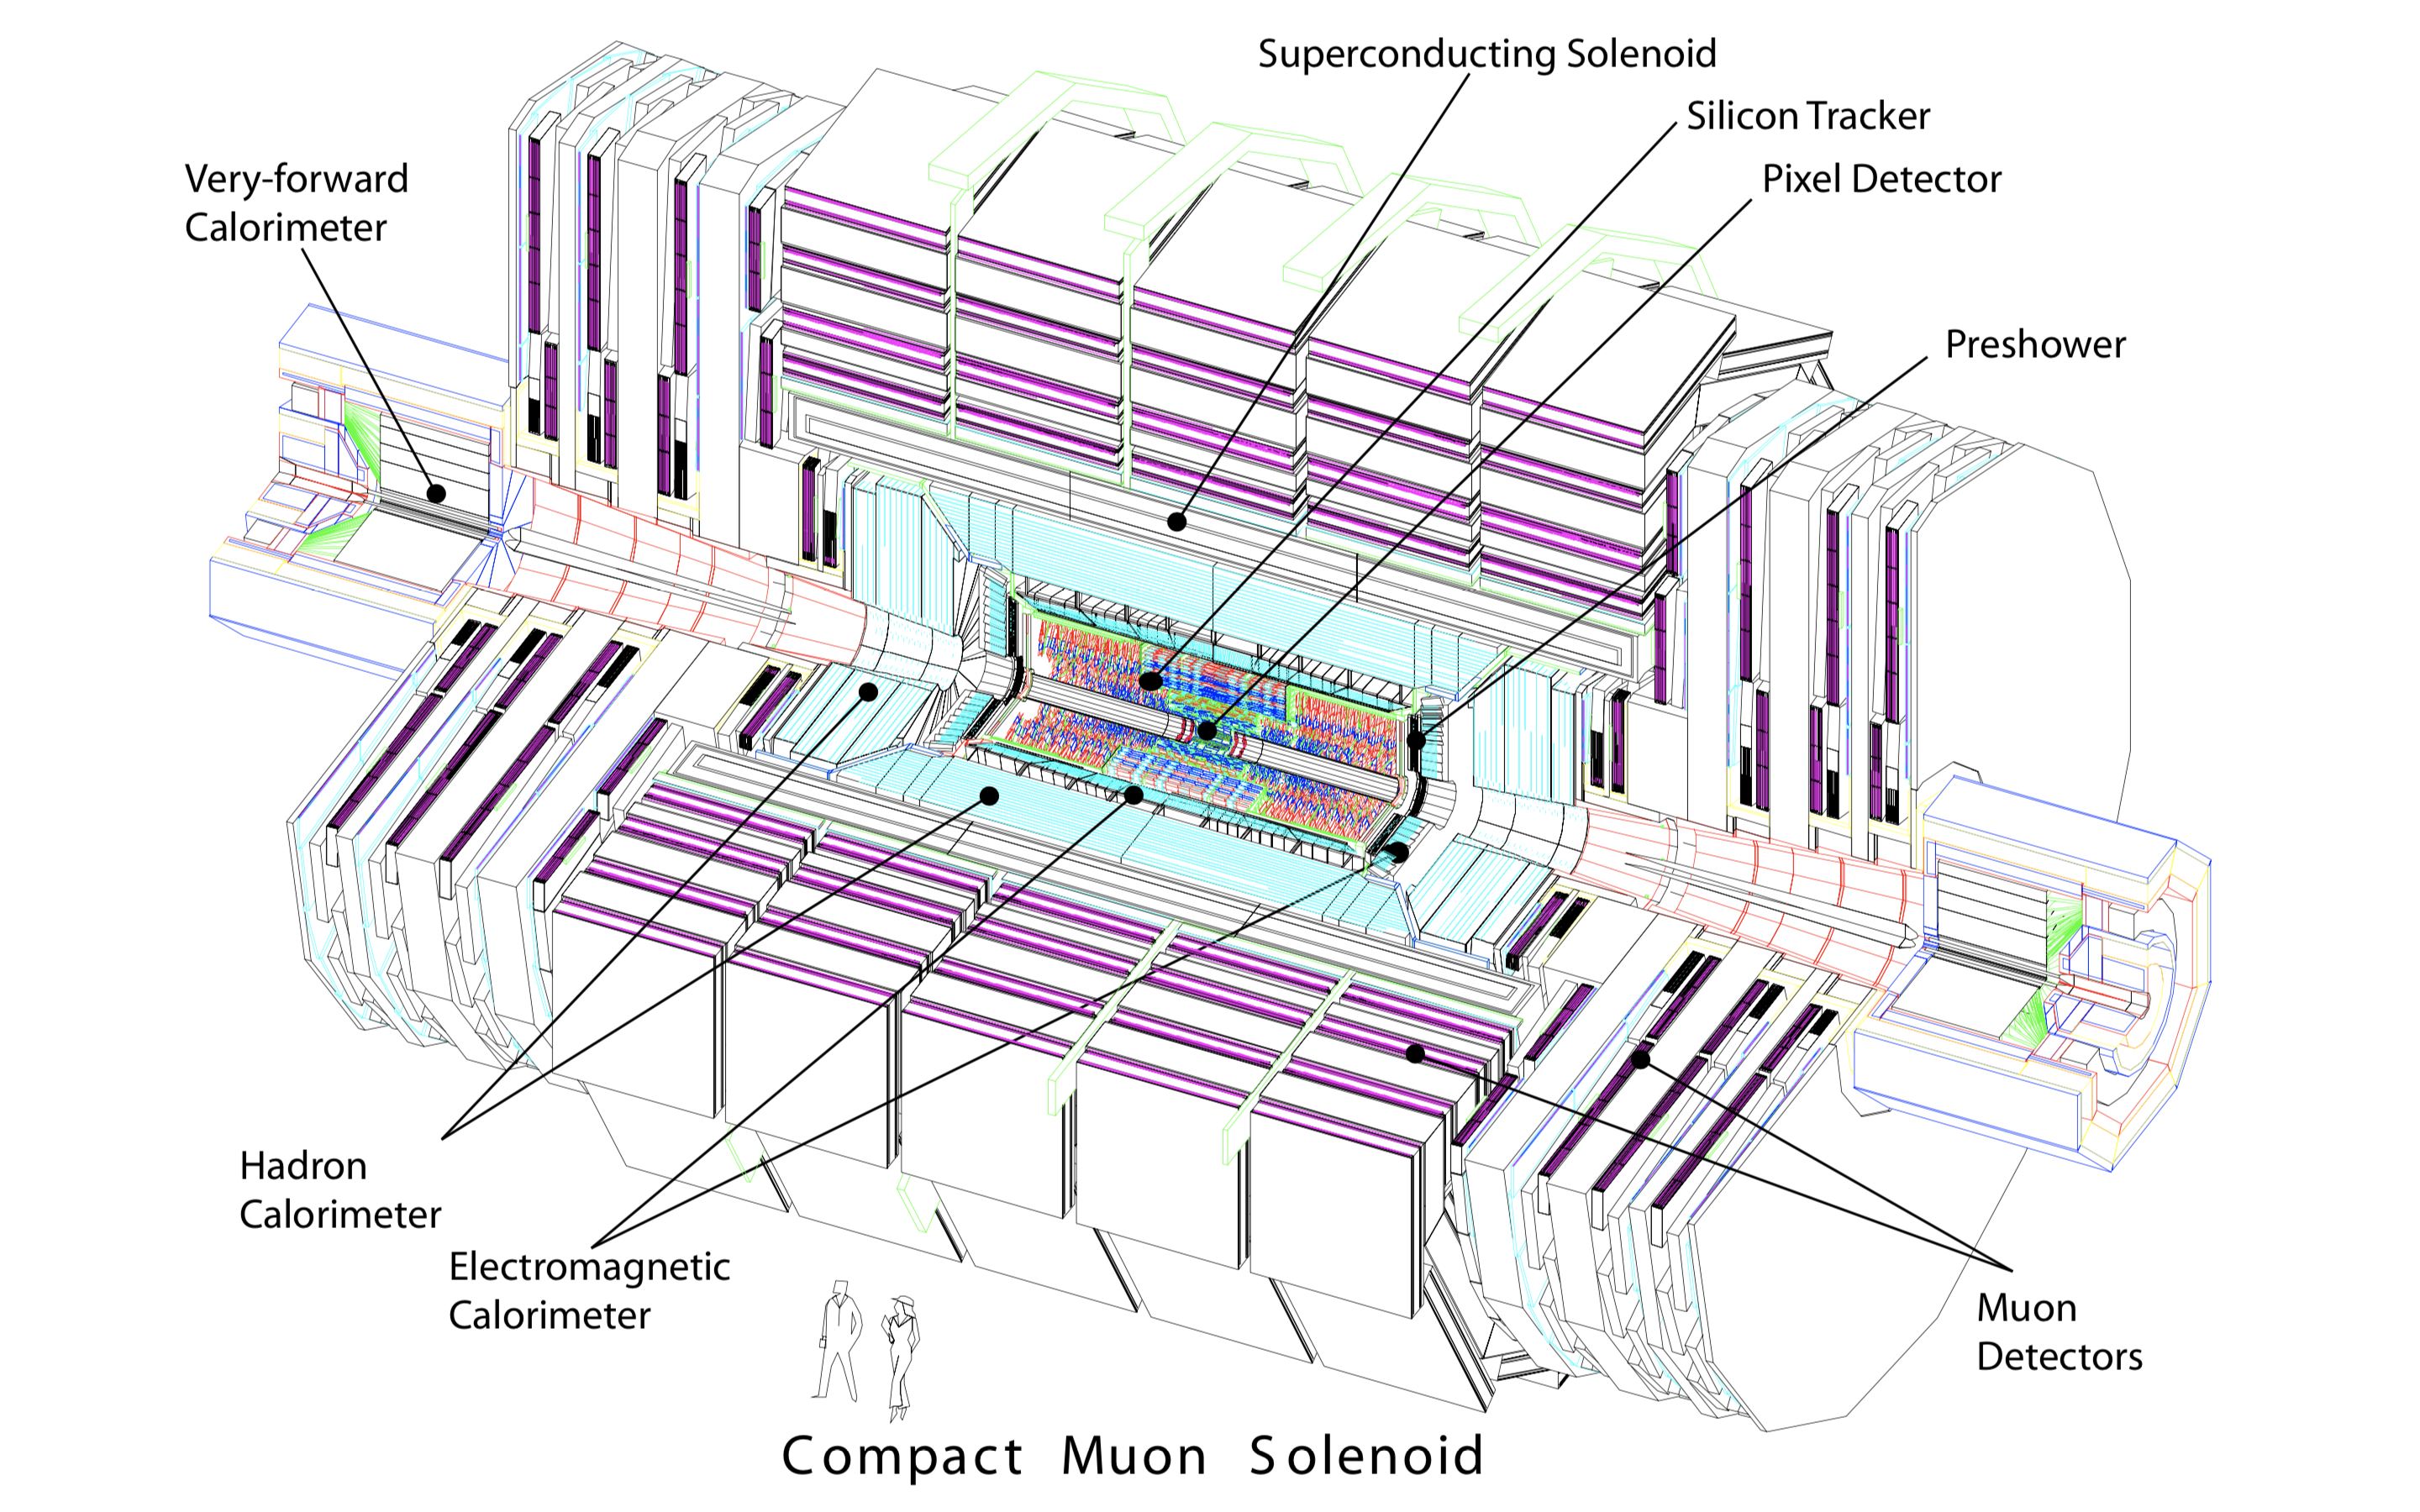
\includegraphics[width=0.8\textwidth]{Figures/ExpApparatus/CMS_detector.png}\\
		\caption{CMS structure\cite{Chatrchyan:2008aa}}
		\label{ExpApp:fig:CMS_structure}
		\end{figure}
		\FloatBarrier

		At the same time, the detector's slices of different functions are shown in Fig.\ref{ExpApp:fig:CMS_slices}(ref.\cite{Barney:2120661})

		\begin{figure}[H]
		\centering{}
	    	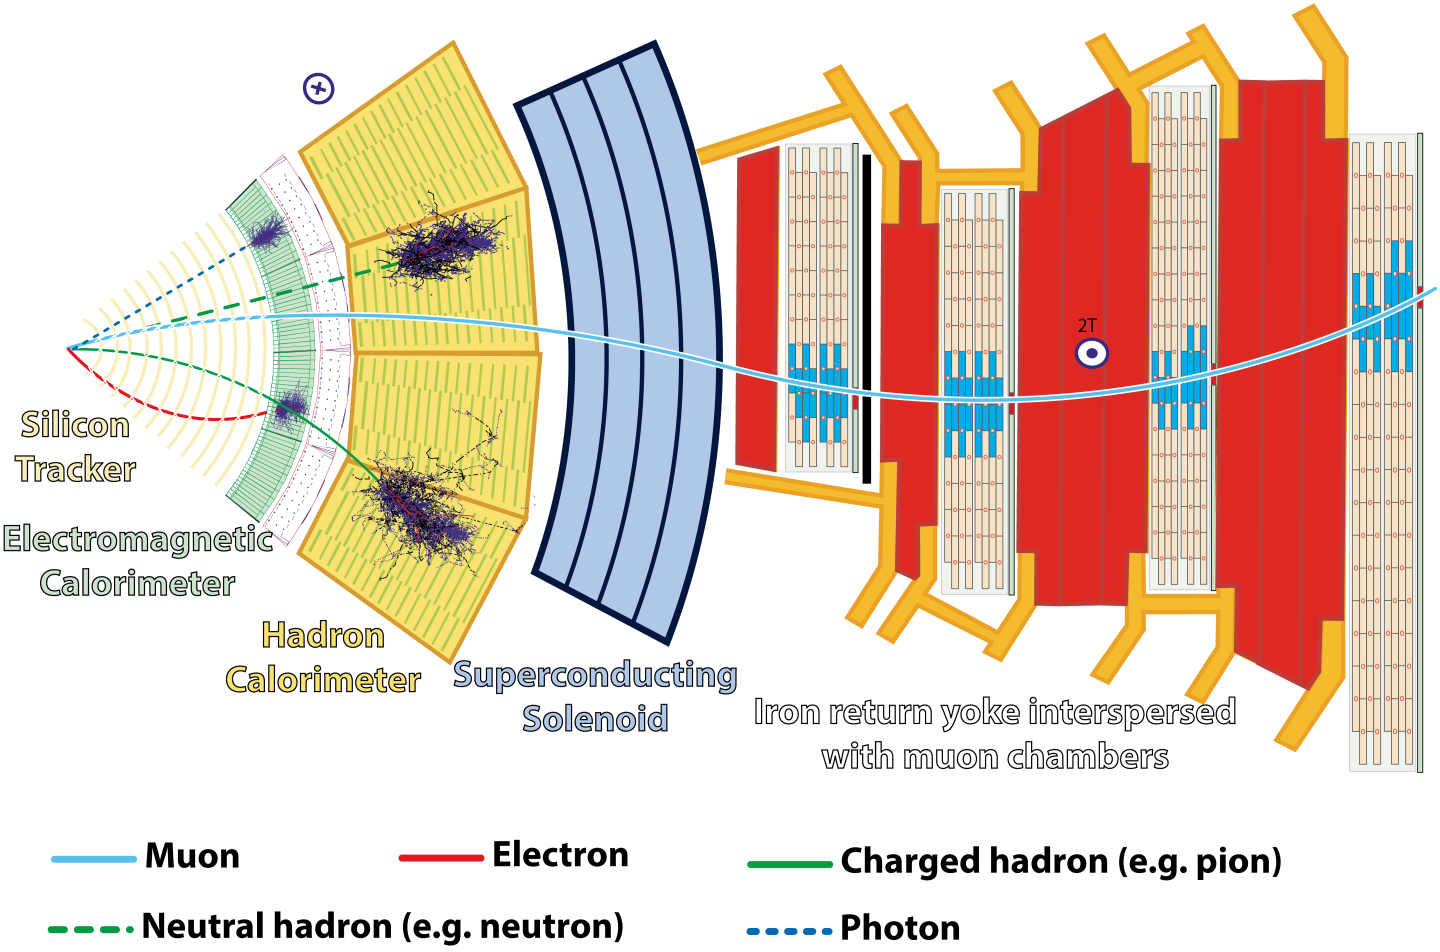
\includegraphics[width=0.8\textwidth]{Figures/ExpApparatus/CMSslice_whiteBackground.png}\\
		\caption{CMS slices\cite{Barney:2120661}}
		\label{ExpApp:fig:CMS_slices}
		\end{figure}
		\FloatBarrier

		The CMS use the right-handed coordinate, that is, the x-axis points to the center of LHC, y-axis points up and orthogonal to the ground, and z-axis is along with anti-clockwise beam direction. The angle $\phi$ is the azimuthal angle on the x-y plane;The other angle $\theta$ means the polar angle which is the angle between the positive z-axis and the observed point. Instead, in LHC the pseudo-rapidity $\eta = -\ln{\tan{(\theta/2)}}$ is more common used because $\eta$ is lorentz invariance under frame transformation. The other usuall usage is the $"$transverse$"$, for example, transvers momentum $p_T$ means the projection of momentum on the x-y plane which is exactly $p_T = \sqrt{p_x^2 + p_y^2}$.

		The different physical objects would be caught by different part of CMS detector. The muon has bended trajectory in tracker and muon chambers but pass without interacting with ECAL; An electron is seen from combined information from tracker(cureved trajectary) and ECAL; A photon is fully deposited on ECAL without reaction passing tracker; The hadrons also have no interaction with track system, but the charged hadron's hadronization and showering could be approached with both ECAL and HCAL.

		\subsubsection{Tracking system}
		\label{sssec:ExpApp_tracking}

			The CMS tracker's schematic drawing is shown below in Fig.\ref{ExpApp:fig:tracker} from reference\cite{Chatrchyan:2014fea} where $\textbf{strip tracker}$ with small silicon tracker within. 

			\begin{figure}[H]
			\centering{}
		    	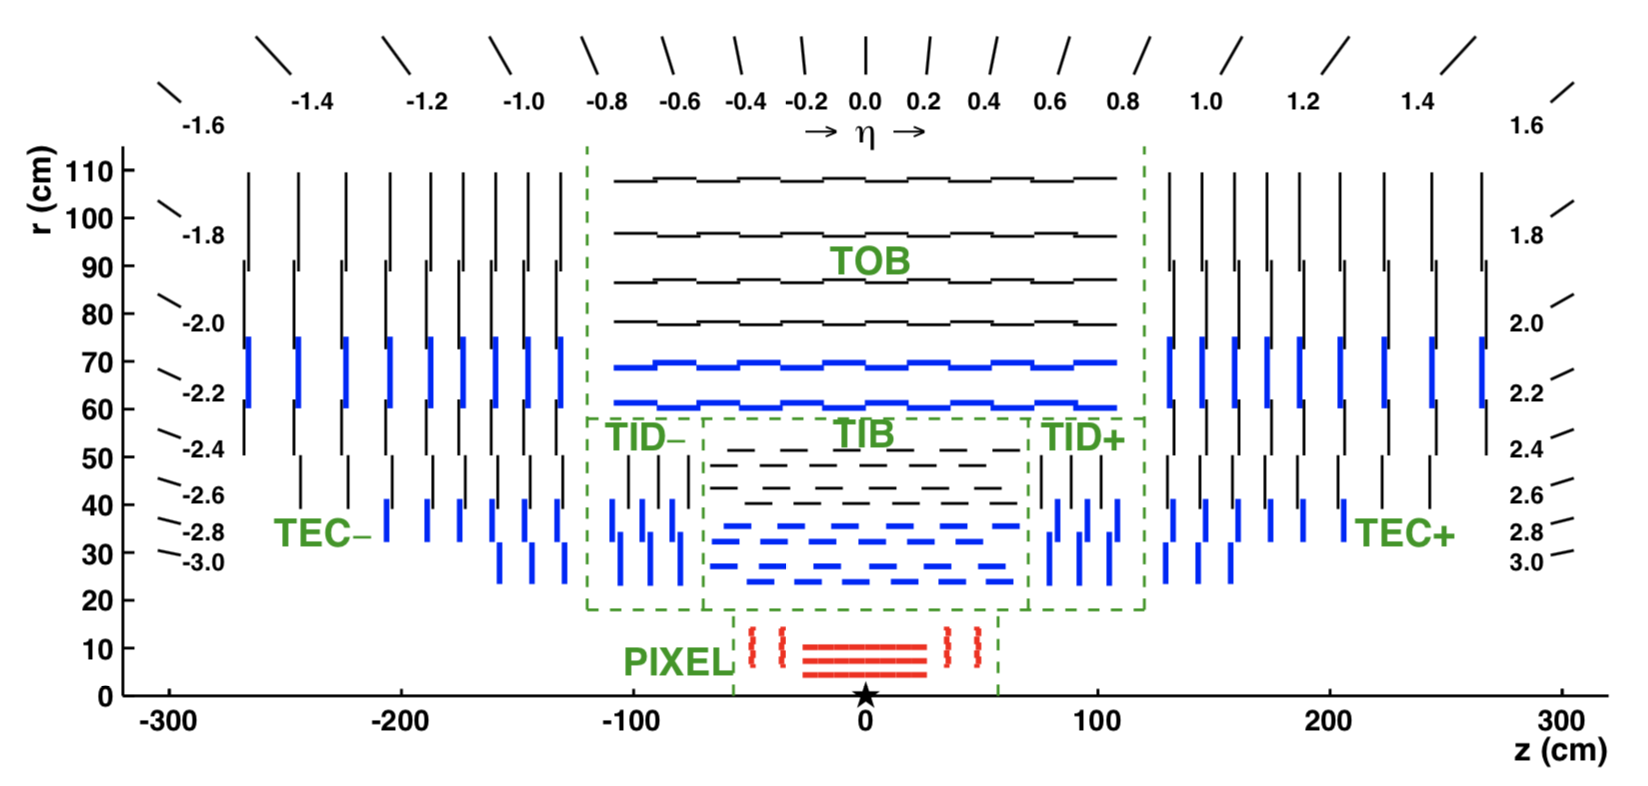
\includegraphics[width=0.85\textwidth]{Figures/ExpApparatus/tracker.png}\\
			\caption{The drawing of the CMS inner tracking system\cite{Chatrchyan:2014fea}}
			\label{ExpApp:fig:tracker}
			\end{figure}
			\FloatBarrier

			Futhermore, the tracker is immersed in magnetic field from CMS solenoid. There are four subsystem in it and they are completed by endcaps(|pseudorapidity $\eta | < 2.5$) on either sides of barrels. The four subsystems are the $\textbf{Tracker}$ $\textbf{Inner}$ $\textbf{Barrel}$$\textbf{(TIB)}$, the $\textbf{Tracker}$ $\textbf{Inner}$ $\textbf{Disk}$$\textbf{(TID)}$, the $\textbf{Tracker}$ $\textbf{Outer}$ $\textbf{Barrel}$$\textbf{(TOB)}$, and the $\textbf{Tracker}$ $\textbf{EndCaps}$$\textbf{(TEC)}$. There are slices of silicons in these tracking subsystems, and the detail of thickness, position and layers would be found in reference\cite{Chatrchyan:2014fea}. Also, the summary of the principal characteristics of the various tracker subsystems from \cite{Chatrchyan:2014fea} is attached below\ref{ExpApp:fig:tracker_sum}:
			
			\begin{figure}[H]
			\centering{}
		    	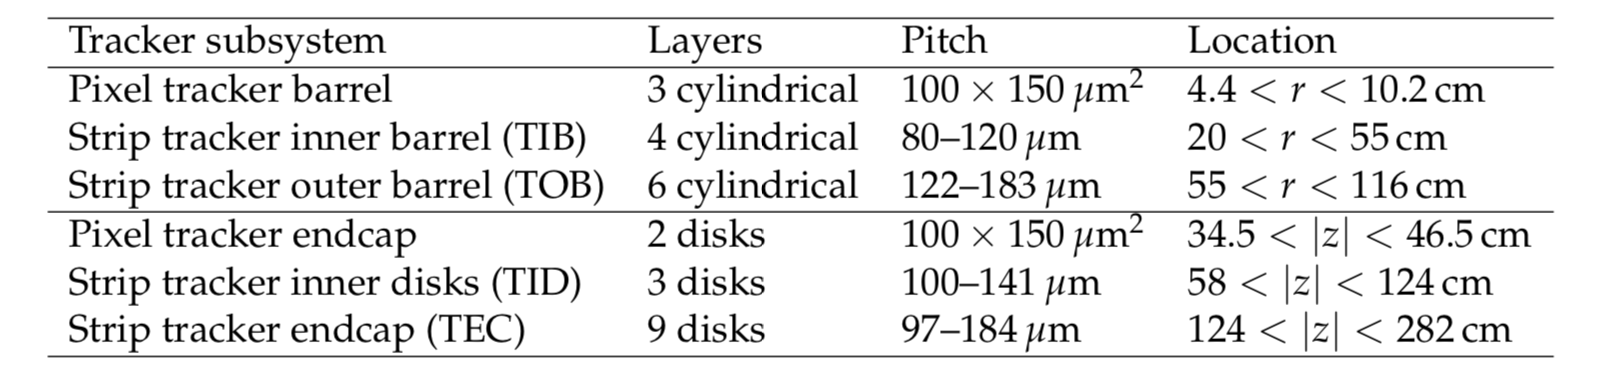
\includegraphics[width=0.85\textwidth]{Figures/ExpApparatus/summary_subtracker.png}\\
			\caption{Summary of the principal characteristics of the various tracker subsystems\cite{Chatrchyan:2014fea}}
			\label{ExpApp:fig:tracker_sum}
			\end{figure}
			\FloatBarrier

		\subsubsection{Electromagnetic Calorimeter(ECAL)}
		\label{sssec:ecal}

			$\textbf{Electromagnetic Calorimeter(ECAL)}$ is a fine-grain, compact, homogeneous calorimeter which is composed of $PbWO_4$ scintillating crystal. Because of its small radiation length, radiation tolerance, and small Molie`re radius, the material is chose. The numerous crystals are arranged in $\textbf{central}$ $\textbf{barrel}$ $\textbf{section}$$\textbf{(EB)}$ and two $\textbf{endcaps}$$\textbf{(EE)}$ respectively. They line in cetral barrel section with the range $|\eta|<1.48$ as quasi-projective pattern. Also, the crystals line in endcaps covering the extensive range up to $|\eta|=3.0$. The transverse size of crystal is appropriate to the shower size in $PbWO_4$, being advantage for photon's shower-shape-based identification. However, $PbWO_4$ has low light yields, so there must be some photodetectors with internal amplification used to get available light yield signal. There are also the $\textbf{preshower}$ $\textbf{detector}$$\textbf{(ES)}$ which are 2 layers of lead absorber. The preshower detector is placed at the range $1.65<|\eta|<2.5$ and in the front side of the endcaps(EE), and the lead avsorbers are installed with orthogonal layers of silicon strip sensors. The main purpose of the preshowerr detector is to help separating $\pi_0$ and $\gamma$. The ECAL structure schemas are shown in Fig.\ref{ExpApp:fig:ECAL1} and Fig.\ref{ExpApp:fig:ECAL2} . The details could be checked in ref.\cite{ECAL_ex}.


			\begin{figure}[H]
			\centering{}
		    	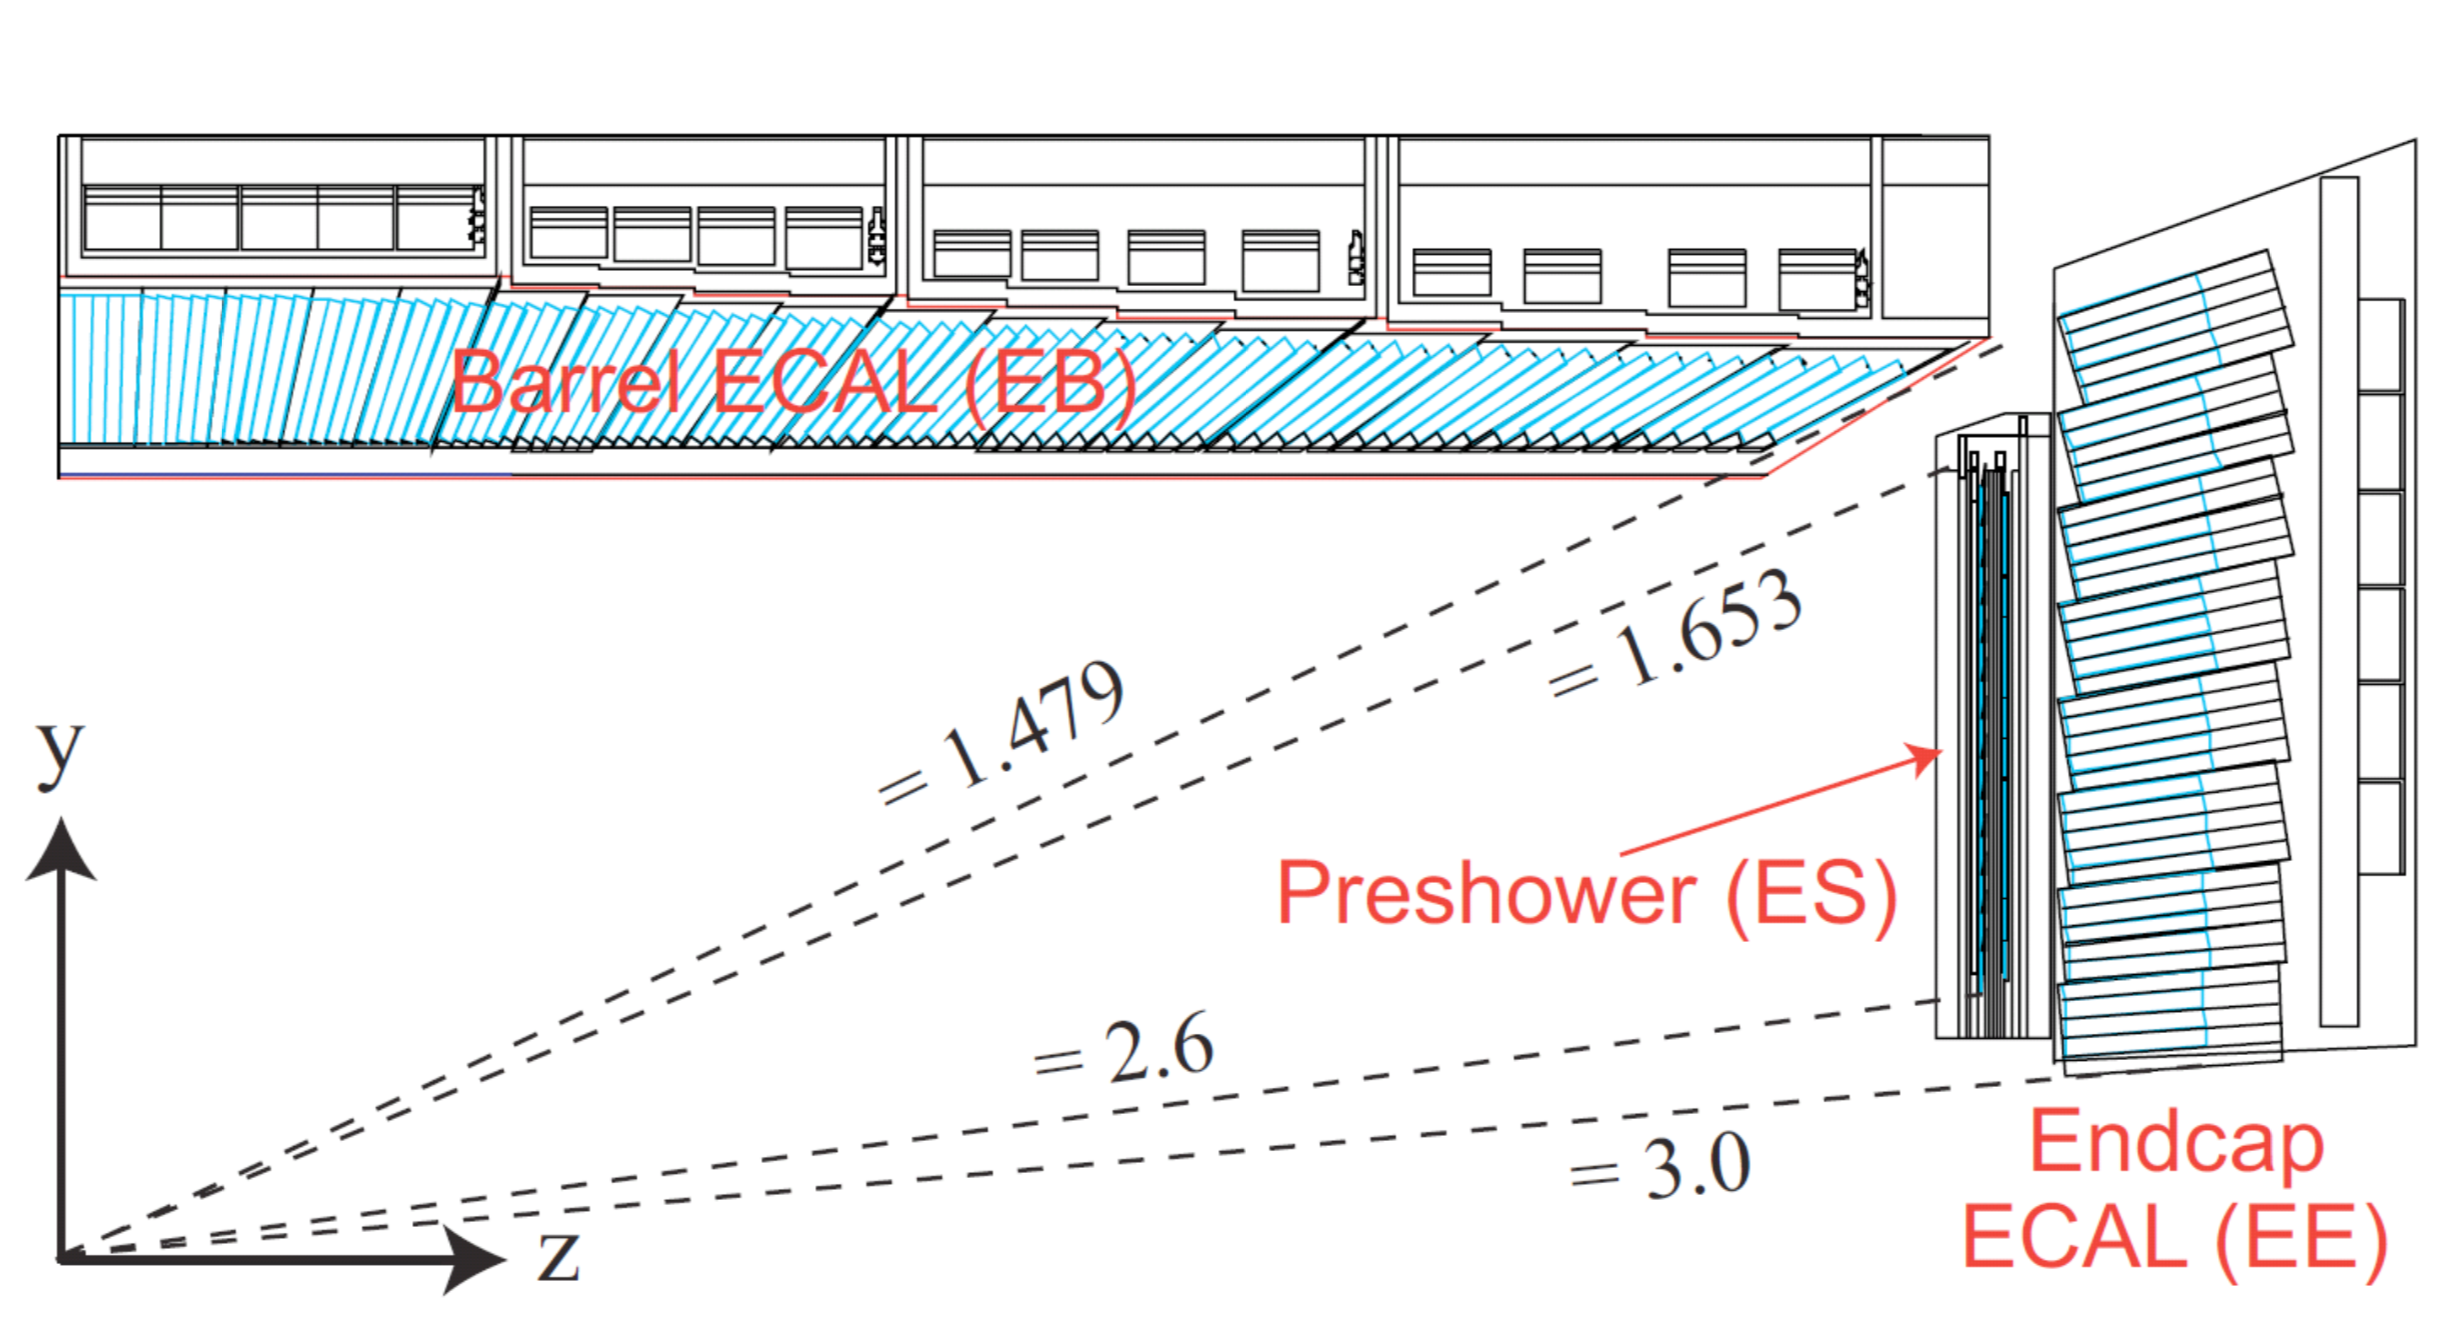
\includegraphics[width=0.85\textwidth]{Figures/ExpApparatus/ECAL.png}\\
			\caption{ECAL structure schema-1\cite{ECAL_ex}}
			\label{ExpApp:fig:ECAL1}
			\end{figure}
			\FloatBarrier

			\begin{figure}[H]
			\centering{}
		    	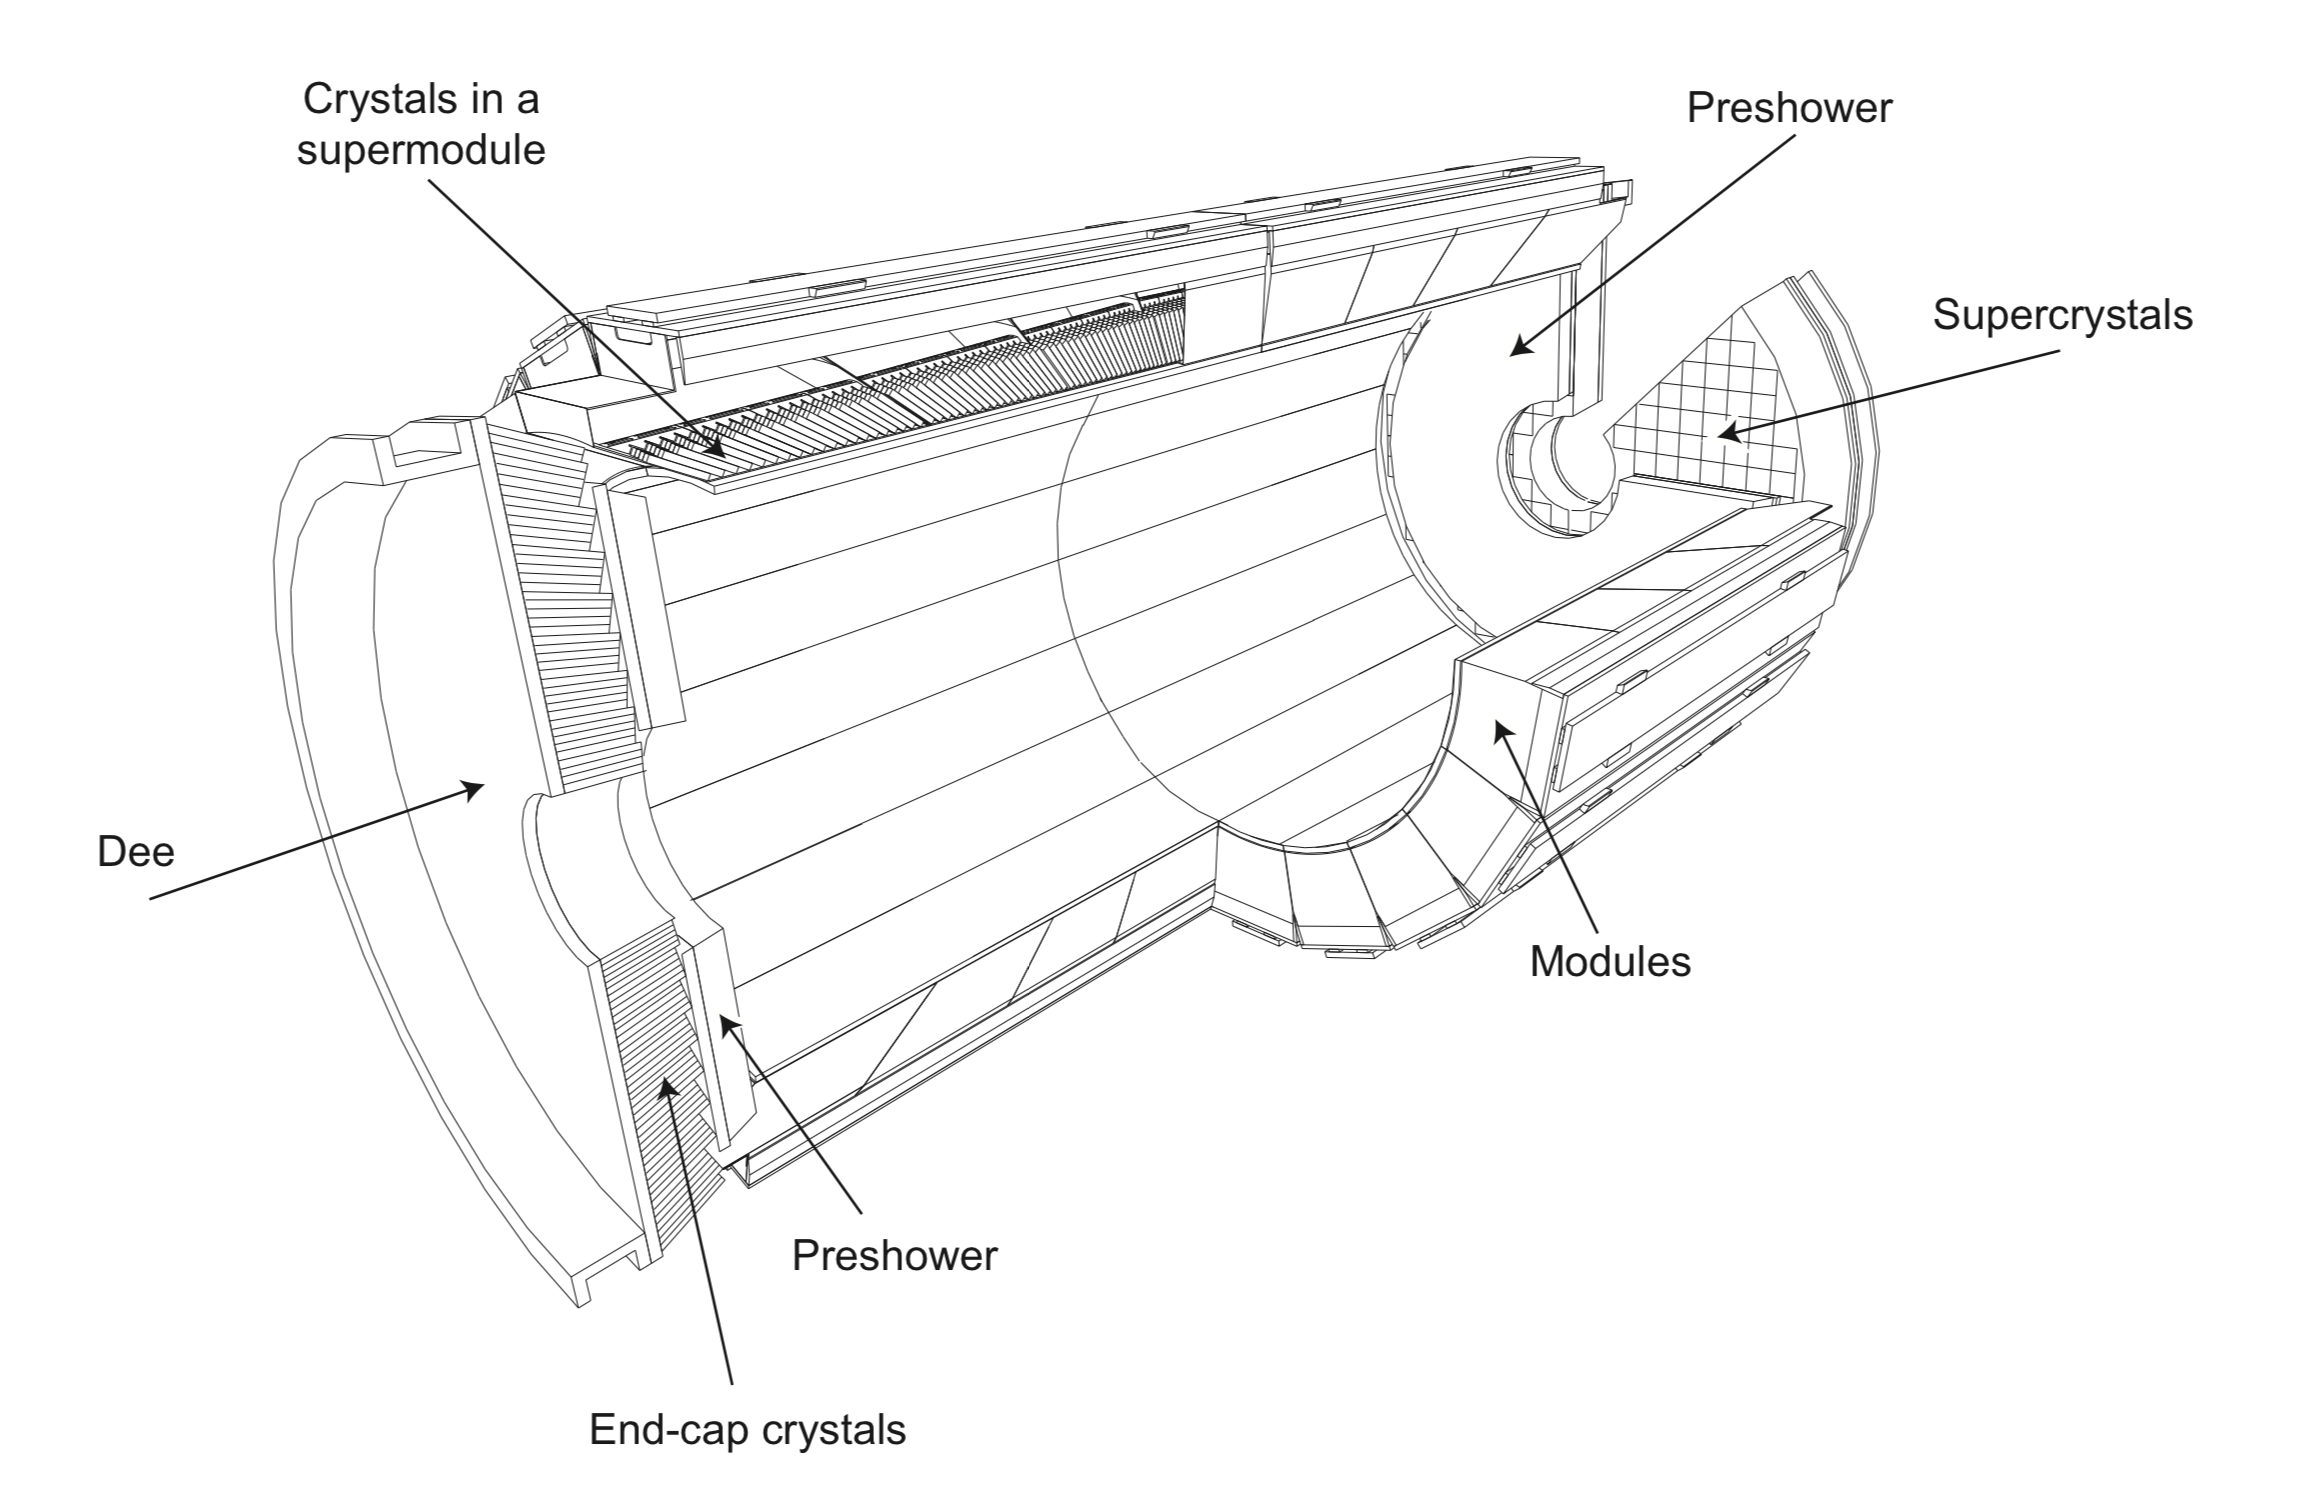
\includegraphics[width=0.85\textwidth]{Figures/ExpApparatus/ECAL2.png}\\
			\caption{ECAL structure schema-2\cite{ECAL_ex}}
			\label{ExpApp:fig:ECAL2}
			\end{figure}
			\FloatBarrier

		\subsubsection{Hadronic Calorimeter(HCAL)}
		\label{sssec:hcal}

			$\textbf{Hadronic Calorimeter(HCAL)}$ contains four subsystems -- the barrel(HB), endcap(HE), outer(HO), and forward(HF) calorimeters.
			\cite{Canko_ak_2009}
			\cite{collaboration_2012}

		\subsubsection{Muon Chambers}
		\label{sssec:muon_detector}

			The highlighting feature of CMS detector is the muon detector. The muon system in CMS is designed to have capacity of reconstructing the momentum and charge of muon completely under the available range of LHC's energy scale. The silicon tracker inside could measure the charge particles' momentum in the range $|\eta|<2.5$. In addition, the muon detector is located outside covering range $|\eta|<2.4$. By collecting positions on the multi-layers of stations and tracker record, the detectors trace the muons' path. The momentum record is based on the concept that the more momentum carried by muon, the less the bending angle of it. For part of hardware, there are 3 types of gaseous detector identifying muons. Those are gas ionization chambers which is appropriate to constitute CMS muon system: $\textbf{drift}$ $\textbf{tube}$ $\textbf{chambers}$$\textbf{(DTs)}$, $\textbf{cathode}$ $\textbf{strip}$ $\textbf{chambers}$$\textbf{(CSCs)}$, and $\textbf{resistive}$ $\textbf{plate}$ $\textbf{chambers}$$\textbf{(RPCs)}$. There are shown in structure diagram in Fig.\ref{ExpApp:fig:muon_chamber1}, the DTs are labeled MB($"$Muon Barrel$"$), the CSCs are labeled ME($"$Muon Endcap$"$), and the RPCs are inlayed in both the barrel and endcaps of CMS detector, so they are labeled RB and RE.

			\begin{figure}[H]
			\centering{}
		    	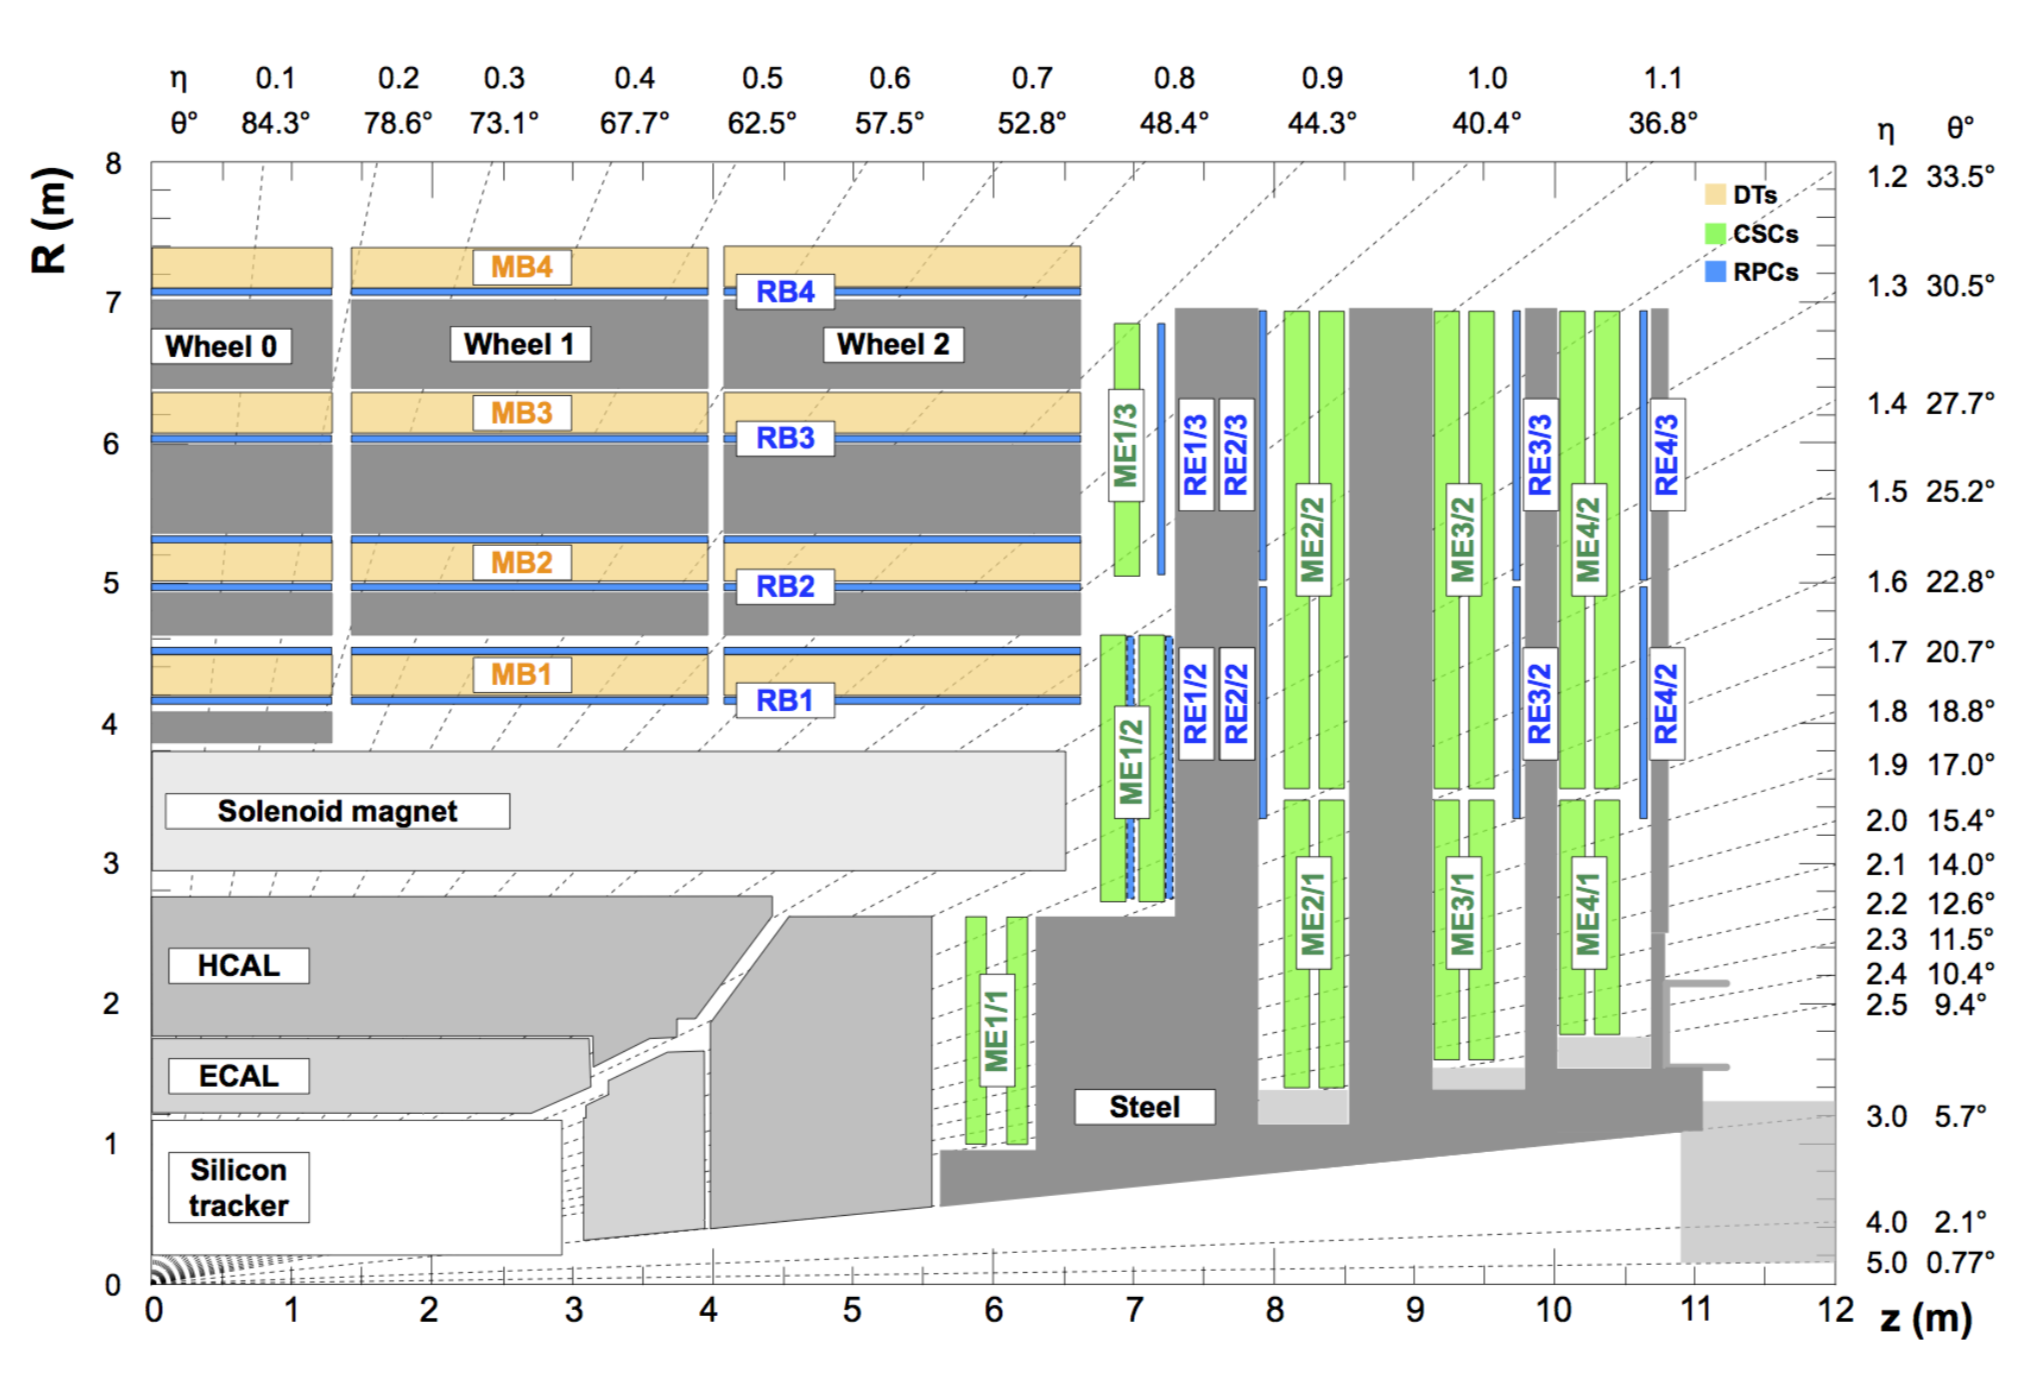
\includegraphics[width=0.75\textwidth]{Figures/ExpApparatus/muon_chamber.png}\\
			\caption{Muon detectors structure\cite{Sirunyan:2018fp}}
			\label{ExpApp:fig:muon_chamber1}
			\end{figure}
			\FloatBarrier

			The DT chambers cover the $\eta < 1.2$ rergion and are organized into four stations. The front three stations contain 8 chambers with 2 set of four chambers. They measured both the muon cooordinate in $\phi - r$ plane(which is equal to x-y plane) and z direction along the beam line. The forth station does the job only for the best angular resolution rather than on z-direction. To eliminate the dead spots in the efficiency, the chamers' drift cells are offset a half-cell width related to their neighbor; In the 2 regions of endcaps, the CSC which is characterized fast response time, fine segmentation, and radiation resistance can deal with high background level and large non-uniform magnetic field at $0.9 < |\eta| < 2.4$. Also with 4 stations perpendicular to beam line, the CSCs arrange radially outward and do the measurement precisely in the x-y plane. Besides, 6 layers of CSC robustly rejects non-muon background and provides efficient matching of hits to other stations and hits in tracker. Those are some of the reason why CMS has great muon-seen performance; The RPCs, which are double-gap chambers, have properties which are fast, independent, and having highly-segmented trigger. The trigger is a steep $p_T$ threshold at the portion of the range $|\eta| < 1.6$ of the muon system. In order to ensure good operating at high rates, avalanche mode would be operated by the chambers. The first 2 layers of 6 layers RPCs in barrel region are designed redundancy to give a low-$p_T$-tracks trigger algorithm which might have stopped before reaching outer stations. Ather structure plot is shown in Fig.\ref{ExpApp:fig:muon_chamber2}.(ref.\cite{Chatrchyan:2008aa},\cite{Chatrchyan:2013sba},\cite{Sirunyan:2018fpa})
		
			\begin{figure}[H]
			\centering{}
		    	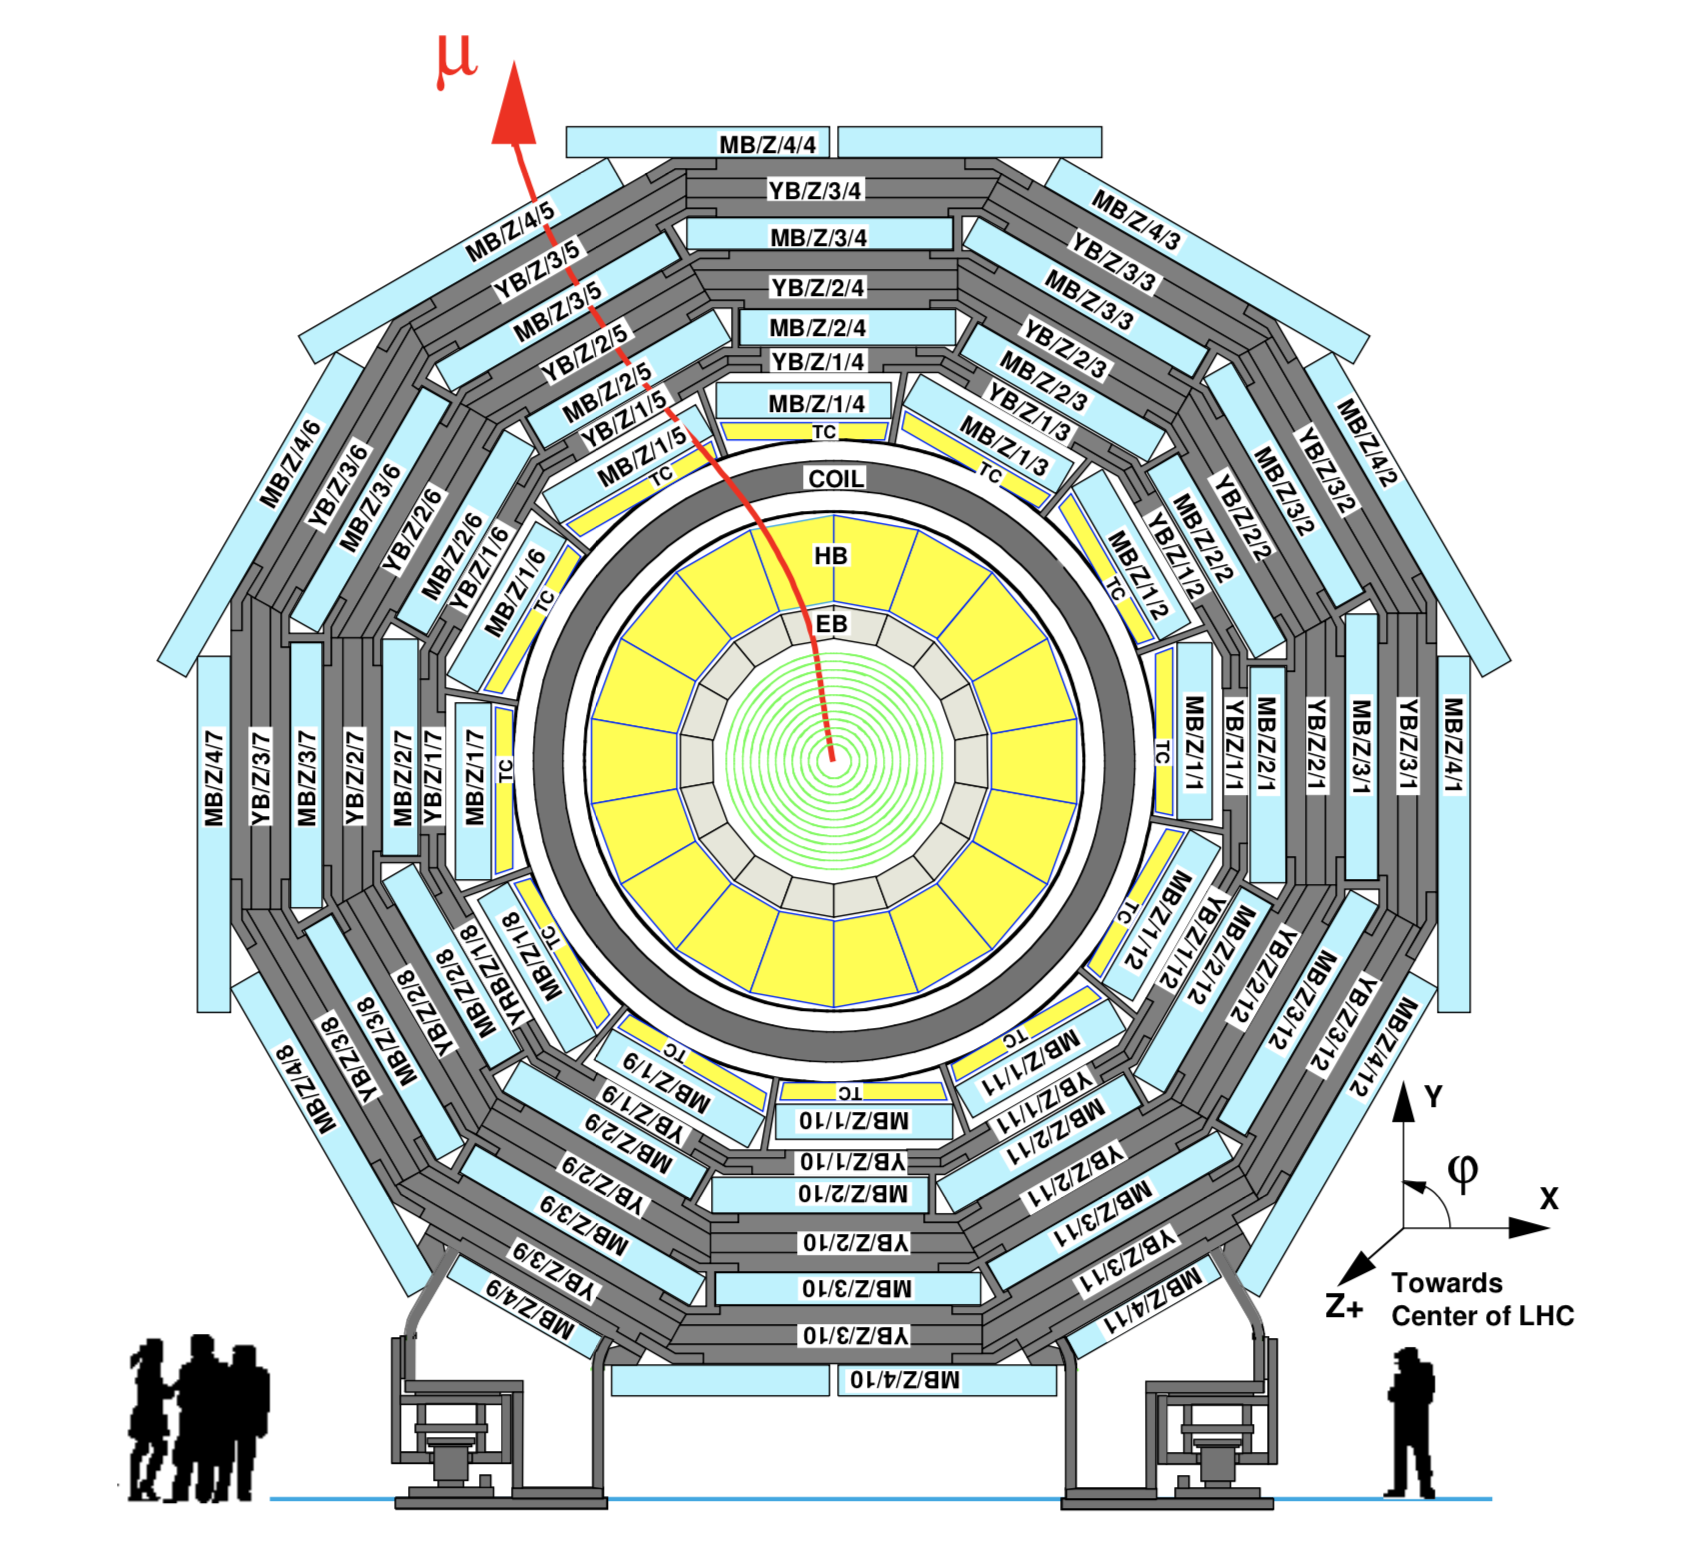
\includegraphics[width=0.75\textwidth]{Figures/ExpApparatus/muon_chamber2.png}\\
			\caption{Muon detectors structure\cite{Chatrchyan:2008aa}}
			\label{ExpApp:fig:muon_chamber2}
			\end{figure}
			\FloatBarrier

			%\cite{Chatrchyan:2008aa} %overview 2008
			%\cite{Chatrchyan:2013sba} % 7tev muon detector
			%\cite{Sirunyan:2018fpa} %reco 13tev




